\documentclass[12pt,letterpaper,fleqn]{article}          % fleqn: align equations left

% File produced by Jeremy West
% This file may be distributed and/or modified:
%   1. under the LaTeX Project Public License and/or
%   2. under the GNU Public License.

% Pretty much required packages for me:
\usepackage{fullpage}                                    % Use the full page
\usepackage{fontspec}
\setmainfont{baskerville}
\usepackage{amsmath}                                     % Math equations, etc.
\usepackage{graphicx}                                    % Enable images (no .eps w/o below option)
\usepackage{epstopdf}                                    % Convert .eps images on the fly
\usepackage{color}                                       % Enables colored text
\definecolor{darkblue}{rgb}{0.0,0.0,0.66}                % Custom color: dark blue
\usepackage[hyperfootnotes=false,bookmarksopen]{hyperref}% Enable hyperlinks, expand menu subtree
\hypersetup{                                             % Custom hyperlink settings
    pdffitwindow=false,                                  % true: window fit to page when opened
    pdfstartview={XYZ null null 1.00},                   % Fits the zoom of the page to 100%
    pdfnewwindow=true,                                   % Links in new window
    colorlinks=true,                                     % false: boxed links; true: colored links
    linkcolor=darkblue,                                  % Color of internal links
    citecolor=darkblue,                                  % Color of links to bibliography
    urlcolor=darkblue  }                                 % Color of external links
\usepackage{booktabs}                                    % For better tables
\newcommand{\ra}[1]{\renewcommand{\arraystretch}{#1}}    % Spacing for tables improved
\renewcommand{\arraystretch}{1.5}                        % Spaces arrays at 1.5x for readability
\usepackage{pdflscape}                                   % Use: \begin{landscape} ... \end{landscape}

% Some "optional" packages that I frequently use:
\usepackage{datetime}                                    % Custom date format for date field
\newdateformat{mydate}{\monthname[\THEMONTH] \THEYEAR}   % Defining month year date format
\usepackage[authoryear]{natbib}                          % Bibliography and citation formating
\usepackage[section]{placeins}                           % Forces floats to stay in section
\usepackage{float}                                       % Used with restylefloat
\restylefloat{figure}                                    % "H" forces a figure to be "exactly here"
\usepackage{textcomp}                                    % Supports many additional symbols
\usepackage{amsthm}                                      % Math theorems, etc.
\usepackage{amsfonts}                                    % Math fonts (e.g. script fonts)
\usepackage{amssymb}                                     % Math symbols such as infinity
\DeclareMathOperator*{\Max}{Max}                         % Better looking max function
\DeclareMathOperator*{\Min}{Min}                         % Better looking min function
\usepackage{subfig}                                      % Enables arrayed images
\usepackage{setspace}                                    % Enables custom margins, doublespacing, etc.
\usepackage{tikz}                                        % Timelines and other drawings
\usetikzlibrary{decorations}                             % Formating for Tikz


\usepackage{color}

\definecolor{mygreen}{rgb}{0,0.6,0}
\definecolor{mygray}{rgb}{0.5,0.5,0.5}
\definecolor{mymauve}{rgb}{0.58,0,0.82}
\definecolor{light-gray}{gray}{0.95}
\usepackage{listings}

\lstdefinestyle{customc}{
backgroundcolor=\color{light-gray},
  belowcaptionskip=1\baselineskip,
  breaklines=true,
  frame=single,
  xleftmargin=\parindent,
  language=C++,
  showstringspaces=false,
  basicstyle=\footnotesize\ttfamily,
  keywordstyle=\bfseries\color{green!40!black},
  %commentstyle=\itshape\color{purple!40!black},
  identifierstyle=\color{blue},
  %stringstyle=\color{orange},
  numberstyle=\tiny\color{mygray},
  numbers=left,                    % where to put the line-numbers; possible values are (none, left, right)
  numbersep=5pt,                   % how far the line-numbers are from the code
  commentstyle=\color{mygreen},
  stringstyle=\color{mymauve},
}

\lstdefinestyle{customasm}{
  belowcaptionskip=1\baselineskip,
  frame=L,
  xleftmargin=\parindent,
  language=[x86masm]Assembler,
  basicstyle=\footnotesize\ttfamily,
  commentstyle=\itshape\color{purple!40!black},
}

\lstset{escapechar=@,style=customc}

\usepackage{titlesec}
\usepackage{lipsum}
\titleformat{\section}
  { \large \normalfont\scshape}{\thesection}{1em}{}
  \titleformat{\subsection}
  { \normalfont\scshape}{\thesection}{1em}{}

  
\newcommand{\horrule}[1]{\rule{\linewidth}{#1}} 	% Horizontal rule

\title{
		%\vspace{-1in} 	
		\usefont{OT1}{bch}{b}{n}
		\normalfont \normalsize \textsc{ \fontspec{Zapfino} King Abdullah University of Science and Technology} \\ [25pt]
		\horrule{0.5pt} \\[0.4cm]
         \Large Fall 2015 CS 247 Scientific Visualization Assignment 2\\
		\horrule{2pt} \\
}

\author{Gang Liao \footnote{Extreme Computing Research Center, Department of Computer Science, King Abdullah University of Science and Technology (KAUST).  Email: \href{mailto:liao.gang@kaust.edu.sa}{liao.gang@kaust.edu.sa}} \hspace{1.05cm}ID: 133267 }

\begin{document}

\maketitle

\onehalfspacing

\section{2D Iso-contours Rendering}
To make sure when you change the slice everything gets updated correctly, before extracting the data, we need to diverge the code segment 
for different \textbf{current\_axis}. 

\begin{lstlisting}
if (current_axis == 0)
{
int x = current_slice[current_axis];
for (int y = 0; y < vol_dim[1] - 1; y+= 1) {
for (int z = 0; z < vol_dim[2] - 1 ; z+= 1) {
	cell = 0;
	if (Data(x, y, z) < current_iso_value - epsilon) cell |= 8;
	if (Data(x, y + 1, z) < current_iso_value - epsilon) cell |= 4;
	if (Data(x, y + 1, z + 1) < current_iso_value - epsilon) cell |= 2;
	if (Data(x, y, z + 1) < current_iso_value - epsilon) cell |= 1;
	GetLinePoints(cell, z, y, vol_dim[2], vol_dim[1], Data(x, y, z), Data(x, y + 1, z), Data(x, y + 1, z + 1), Data(x, y, z + 1));			
	}}
}				
\end{lstlisting}

Since there exists 16 intersected models in 2D cells, it can be reduced to 8.  I set \textbf{edgeTable2D} as:

\begin{lstlisting}
static char edgeTable2D[16] = {
// ============================================
// TODO: fill marching squares table
// ============================================
	0x0, 0x01, 0x02, 0x03, 0x04, 0x05, 0x06, 0x07,
	0x07, 0x06, 0x05, 0x04, 0x03, 0x02, 0x01, 0x0
//To recognise the same intersected models	
};				
\end{lstlisting}

That's can be used to interpolate the positions of vertices in specified edges. All pairs of vertices are pushed into C++ Vector \textbf{contour}.
In order to find the correct position in the screen, their position should be scaled via right aspect.
\begin{lstlisting}
for (int i = 0; i < contour.size(); i += 4)
{
	x1 = contour[i] * h;
	y1 = contour[i + 1] * w;
	x2 = contour[i + 2] * h;
	y2 = contour[i + 3] * w;

	glColor3f(1.0, 0.0, 0.0);
	glLineWidth(5);
	glBegin(GL_LINES);
	glVertex2d(y1, x1);
	glVertex2d(y2, x2);
	glEnd();
}
\end{lstlisting}
\newpage
\subsection{Result}

\begin{figure}[!htb]
\centering
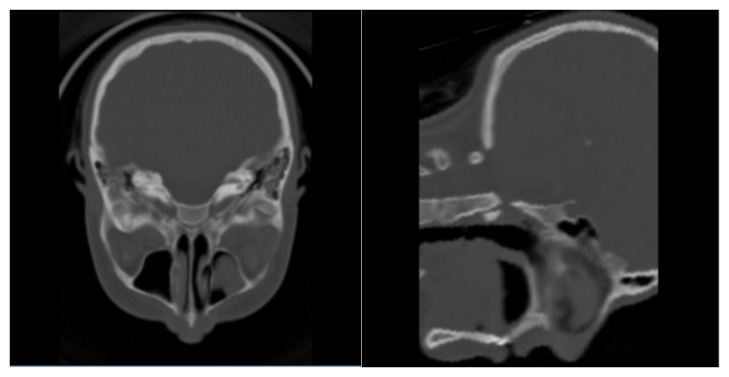
\includegraphics[scale=0.82]{1.pdf}
\end{figure}





\section{3D Iso-surface Rendering}
3D Iso-surface algorithm is similar to 2D Iso-contour. First, we need to get 8 points (virtual cube) according to current points' neighbors. Then, calculating cube index via the specified vertices inside or outside of iso value.
\begin{lstlisting}
cubeindex = 0;
if (cube.val[0] < isolevel) cubeindex |= 1;
if (cube.val[1] < isolevel) cubeindex |= 2;
if (cube.val[2] < isolevel) cubeindex |= 4;
if (cube.val[3] < isolevel) cubeindex |= 8;
if (cube.val[4] < isolevel) cubeindex |= 16;
if (cube.val[5] < isolevel) cubeindex |= 32;
if (cube.val[6] < isolevel) cubeindex |= 64;
if (cube.val[7] < isolevel) cubeindex |= 128;
\end{lstlisting}
Pre-defined \textbf{edgeTable} includes which pair of vertices should be interpolated in bits. Finally, we can get all vertices for triangles via   \textbf{triTable}. 
\begin{lstlisting}
std::vector<float> trian;
for (i = 0; triTable[cubeindex][i] != -1; i += 3)
{
float x1 = vertlist[triTable[cubeindex][i]].x;
float y1 = vertlist[triTable[cubeindex][i]].y;
float z1 = vertlist[triTable[cubeindex][i]].z;
float x2 = vertlist[triTable[cubeindex][i+1]].x; ... //also float y2, z2
float x3 = vertlist[triTable[cubeindex][i+2]].x; ... //also float y3, z3
//store normal per triangle into normal vector
normal.push_back(TriangNorm(vertlist[triTable[cubeindex][i]], vertlist[triTable[cubeindex][i + 1]], vertlist[triTable[cubeindex][i + 2]]));
trian.clear();
trian.push_back(x1); ...//also store y1, z1
trian.push_back(x2); ...//also store y2, z2
trian.push_back(x3); ...//also store y3, z3
//store triangle into iso-surface vector for post-rendering
isosurface.push_back(trian); 
}
\end{lstlisting}


\begin{figure}[!htb]
\centering
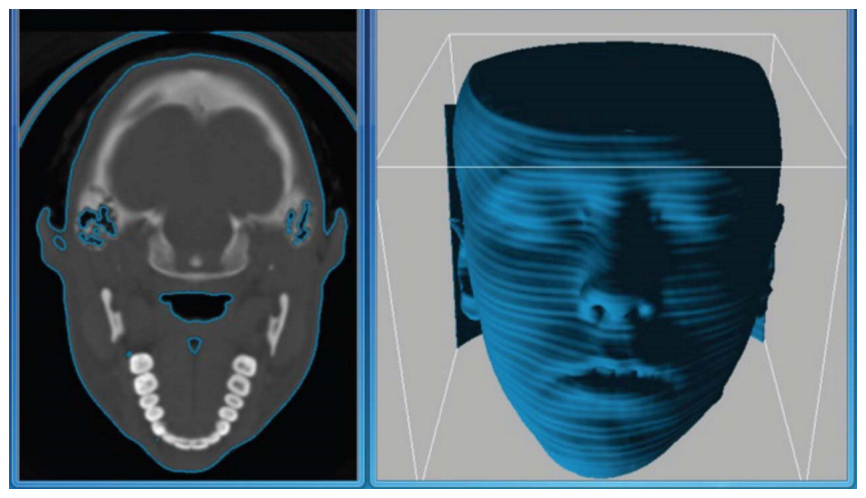
\includegraphics[scale=0.82]{2.pdf}
\end{figure}

\begin{figure}[!htb]
\centering
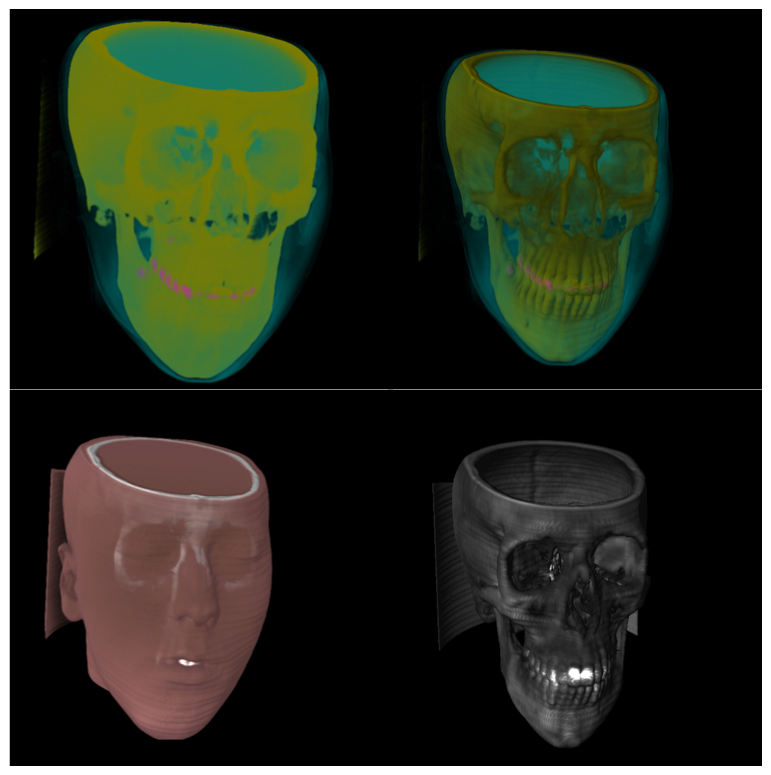
\includegraphics[scale=0.82]{3.pdf}
\end{figure}
%%%%%%%%%%%%%%%%%%%%%%%%%%%%%%%%%%%%%%%%%%%    REFERENCES
%\clearpage
%\singlespacing
%\bibliographystyle{plainnat}
%\bibliography{filename} % Name of .bib references file
%\clearpage

%\vspace{3cm}

%%%%%%%%%%%%%%%%%%%%%%%%%%%%%%%%%%%%%%%%%%%    TABLES & FIGURES
%\newpage
%\section{Tables and Figures}\label{sec:tables}


%%%%%%%%%%%%%%%%%%%%%%%%%%%%%%%%%%%%%%%%%%%    APPENDIX
%\newpage
%\appendix
%\section{Appendix}\label{sec:appendix}


\end{document}
